\documentclass[a4paper]{article}

%% Language and font encodings
\usepackage[english]{babel}
\usepackage[utf8x]{inputenc}
\usepackage[T1]{fontenc}

%% Sets page size and margins
\usepackage[a4paper,top=3cm,bottom=2cm,left=3cm,right=3cm,marginparwidth=1.75cm]{geometry}

%% Useful packages
\usepackage{amsmath}
\usepackage{graphicx}
\usepackage[colorinlistoftodos]{todonotes}
\usepackage[colorlinks=true, allcolors=blue]{hyperref}
\title{Solving Imcompressible Flow by Mixed Finite Element Method}
\author{Quanhui Zhu}

\begin{document}
\maketitle

\begin{abstract}
  This project discusses how to solve Navier-Stokes equations by mixed
  element methods. It begins with the Stokes equations solver, and
  also its AMG block precondition skills; then a Newton iteration is
  designed to deal the nonlinear discretized system of Navier-Stokes
  equations.  For large viscosity parameters ($\geq 0.02$, or RE$\leq
  50$), the solutions of steady Navier-Stokes equations can be solved
  directly by using an ILU preconditioner, while for the small ($\geq
  0.0005$, or RE$\leq 2000$) cases, a time dependent Navier-Stokes
  solver is implemented to approximate the steady solution by making
  the computing time sufficient large. A series bentchmark simulations
  are fulfiled to check the correctness of the algorithms and codes.
\end{abstract}


\section{Stokes Equations}

\subsection{Weak Form}

The Stokes equations we discussed take the form as
\begin{equation}
\begin{array}{rcl}
-\nabla^2 \vec{u} + \nabla p &=& \vec{0} \\
\nabla \cdot \vec{u} &=& \vec{0}
\label{eq::Stokes-problem}
\end{array}
\end{equation}
The equations (\ref{eq::Stokes-problem}) are the fundamental model of
viscous flow with boundary values considered that
\begin{equation}
\vec{u} = \vec{w} \ on \ \partial \Omega_D ,\quad \frac{\partial
  \vec{u}}{\partial n} - \vec{n} p = \vec{s} \ on \ \partial \Omega_N.
\end{equation}
Here the variable $p$ is the pressure.

We use the P2-P1 mixed elements, or famous as Taylor-Hood elements
\cite{Lee2005Finite} to discrete the equations. And the weak form of
the equations (\ref{eq::Stokes-problem}) reads
\begin{equation}
\begin{array}{rcl}
-\int_\Omega \nabla^2 \vec{u} \cdot \vec{v} + \nabla p &=& 0\\
\int_\Omega q\nabla \cdot \vec{u} &=&0
\label{eq::Stokes-weakform}
\end{array}
\end{equation}

It can be reformed by applying Green Theorem as
\begin{equation}
\begin{array}{rcl}
\int_\Omega \nabla \vec{u} : \nabla \vec{v} - \int_\Omega p\nabla
\cdot \vec{v} &=& \int_{\partial \Omega_N}\vec{s}\cdot \vec{v}, 
\forall \vec{v} \in H^1_{E_0}\\ \int_\Omega q\nabla \cdot \vec{u}
&=& 0, \forall q \in L_2(\Omega)
\label{eq::Stokes}
\end{array}
\end{equation}

Assume that the basis functions of the velocity space are
{$\vec{\phi}_j$} such that
\begin{equation}
\vec{u}_h = \sum^{n_u}_{j=1}u_j\vec{\phi}_j,
\label{eq::Stokes-u}
\end{equation}
while the basis functions of the pressure space are $\psi_k$ such that
\begin{equation}
p_h = \sum^{n_p}_{k=1}p_k\psi_k,
\label{eq::Stokes-p}
\end{equation}
then the weak form can be expressed by the following linear system:
\begin{equation}
\left[ \begin{array}{ccc}
A & B^T \\
B & 0
\end{array}
\right]
\left[\begin{array}{ccc}
u\\
p
\end{array}
\right]=
\left[\begin{array}{ccc}
f\\
g
\end{array}
\right],
\label{mt::Stokes}
\end{equation}
where the matrix $A$ and $B$ are given by
\begin{equation}
\begin{array}{rcl}
A &=& [a_{ij}], \quad a_{ij} = \int_{\Omega} \nabla \vec{\phi}_i :
\nabla \vec{\phi}_j,\\ B &=& [b_{kj}], \quad b_{kj} = -\int_{\Omega}
\psi_k\nabla \cdot \vec{\phi_j},
\end{array}
\end{equation}
respectively.


\subsection{Matrix Form}

Specially, we set the \{$\vec{\phi}_i$\} a standard basis functions that
\begin{equation}
\{\vec{\phi_1},\vec{\phi_2},\cdots,\vec{\phi_{2n}} \}:=\{(\phi_1,0)^T,\cdots,(\phi_n,0)^T,(0,\phi_1)^T,\cdots,(0,\phi_n)^T\}
\label{eq::basisfunction}
\end{equation}
With $u:=([u_x]_1,\cdots,[u_x]_n,[u_y]_1,\cdots,[u_y]_n)$, system (\ref{mt::Stokes}) can be rewritten as
\begin{equation}
\left[ \begin{array}{ccc}
A & 0 & B_x^T \\
0 & A & B_y^T \\
B_x & B_y & 0
\end{array}
\right]
\left[\begin{array}{ccc}
u_x\\
u_y\\
p
\end{array}
\right]=
\left[\begin{array}{ccc}
f_x\\
f_y\\
g
\end{array}
\right]
\label{Stokes}
\end{equation}
where the $n_u \times n_u $ matrix $A$ is the scalar Laplacian matrix, and the $n_p\times n_u$ matrices $B_x$ and $B_y$ represent weak derivatives in the $x$ and $y$ direction that 	
\begin{equation}
\begin{array}{rcl}
A &=& [a_{ij}], \quad a_{ij} = \int_{\Omega} \nabla \phi_i : \nabla \phi_j \\
B_x &=& [b_{x,ki}], \quad b_{x,ki} = -\int_{\Omega} \psi_k \frac{\partial \phi_i}{\partial x} \\
B_y &=& [b_{y,kj}], \quad b_{y,kj} = -\int_{\Omega} \psi_k \frac{\partial \phi_j}{\partial y} \\
\end{array}
\label{Stokes-mtvalue}
\end{equation}
 \\
\subsection{Precondition}
Obviously the matrix system is symmetric positive definite and highly
sparse. Thus proper precondition is needed to improve computing
efficiency. There is a AMG block preconditioner for the Stokes
matrix. The precondition matrix is
\begin{equation}
M = \left[ \begin{array}{ccc}
A & 0 & 0 \\
0 & A & 0 \\
0 & 0 & Q
\end{array}
\right],
\end{equation}
where $Q$ is a $n_p\times n_p$ the mass matrix in the pressure space, which
\begin{equation}
Q = [q_{ij}], \quad q_{ij} = \int_{\Omega} \psi_i\psi_j.
\label{pr::Q}
\end{equation}

In practise, we may just take the diagonal elements of $Q$ since it is
a diagonally dominant matrix. And for the stiff matrix A can be solved
by a standard AMG solver.

\subsection{Numerical Results}
For the first simulation to test our Stokes solver, the dimension of
the computational area is $\Omega = [0,1]\times[0,1]$, and the
boundary values take as following:
\begin{equation}
\left\lbrace
\begin{array}{ll}
u_x = 1, u_y = 0, & y = 1 \\
u_x = u_y = 0, & \mbox{others}.
\end{array}
\right.
\label{bd::value1}
\end{equation}

And the dimension of the mesh grids is about $20 \times 20$, or
$h=0.05$. All the simulations in this report are implemented based on
numerical software lib AFEPack and dealII 8.1.0. 

\begin{figure}[h]
\centering
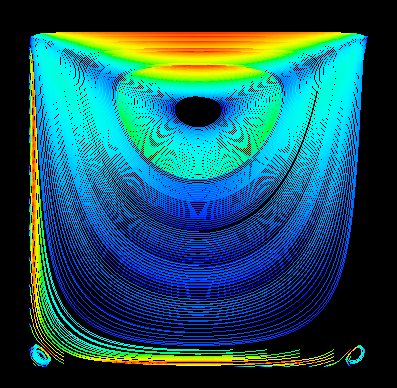
\includegraphics[scale = 0.4]{images/Stokes.png}
\caption{Stokes Solution, the stream lines of the velocity field, the
  size of the square is $[0, 1] \times [0, 1]$, with mesh dimension $h = 0.05$.}
\label{im::Stokes-Solution}
\end{figure}

The Figure \ref{im::Stokes-Solution} shows the streamlines of the
velocity, and the locations of the two counter-rotating recirculations
(called Moffatt eddies) agreed with the ture solutions well.  

\section{Navier Stokes}
\subsection{Weak Form}
Consider the Navier-Stokes equations:
\begin{equation}
\begin{array}{rcl}
-\nu \nabla^2 \vec{u} + \vec{u}\cdot \nabla \vec{u} + \nabla p &=& \vec{F} \\
\nabla \cdot \vec{u} &=& \vec{0}
\label{eq::Navier-Stokes-problem}
\end{array}
\end{equation}
As we did before, a standard weak form is given that
\begin{equation}
\begin{array}{rcl}
-\nu\int_\Omega \nabla^2 \vec{u} \cdot
\vec{v} + \int_{\Omega} \vec{u} \cdot \nabla \vec{u} \cdot \vec{v} + \nabla p
& = & \int_{\Omega} \vec{F} \cdot \vec{v}, \quad \forall \vec{v} \in
H^1_{E_0}, \\ \int_\Omega q \nabla \cdot \vec{u} & = & 0, \quad \forall q
\in L_2(\Omega).
\label{eq::Navier-Stokes-weakform}
\end{array}
\end{equation}
% origin: The problem can't be solved directly...
% the conclusion is incorrect, can not be solved linearly not means can not be solved.
% and in the above formation, you still ommit the interpunctions.
And a newton iteration
$$
x_{n+1} = x_{n} - (A(x_n)-b) \cdot J(A(x_{n}))^{-1}
$$ is considered to solve this nonlinear equations. Here $J(A)$ means
$A$'s Jacobi matrix. The iteration form comes that
$$
J(A(x_n))\Delta x = b - A(x_n).
$$

% why indent again?

It leads to a matrix system similar as the Stokes one with the same
basis functions (\ref{eq::basisfunction}), which is
\begin{equation}
\left[ \begin{array}{ccc}
\nu A + N + W_{xx} & W_{xy} & B_x^T \\
W_{yx} & \nu A + N + W{yy} & B_y^T \\
B_x & B_y & 0
\end{array}
\right]
\left[\begin{array}{ccc}
\Delta u_x\\
\Delta u_y\\
\Delta p
\end{array}
\right] =
\left[\begin{array}{ccc}
f_x\\
f_y\\
g
\end{array}
\right],
\label{Navier-Stokes}
\end{equation}
where the matrix $N$ is the $n_u \times n_u$ scalar convection matrix, which takes the form 
\begin{equation}
N = [n_{ij}], n_{ij} = \int_{\Omega} (\vec{u}_h\cdot \nabla\phi_j)\phi_i,
\label{mt::N}
\end{equation}
and the $n_u\times n_u$ matrices $W_{xx}, W_{xy}, W_{yx}, W_{yy}$
represent weak partial derivatives of the current velocity, which take the form
\begin{equation}
W_{xy} = [w_{xy,ij}], w_{xy,ij} = \int_{\Omega} \frac{\partial u_x}{\partial y}\phi_u \phi_j.
\label{mt::W}
\end{equation}
In the iteration, the nonlinear residual is
\begin{equation}
\begin{array}{rcl}
f &=& [f_i], f_i = \int_{\Omega}(\vec{F} \cdot \vec{\phi}_i -
\vec{u}_h \cdot \nabla \vec{u}_h \cdot \vec{\phi}_i - \nu \nabla
\vec{u}_h : \nabla \vec{\phi}_i + p_h(\nabla \cdot \vec{\phi}_i)), \\ g
& = & [g_k], g_k = \int_{\Omega} \psi_k(\nabla \cdot \vec{u}_h).
\end{array}
\end{equation}

Especially, for $f$ in $x$ and $y$ directions, they are
\begin{equation}
\begin{array}{rcl}
f_x & = & [f_{xi}], f_{xi} = \int_{\Omega}(F_x \cdot \phi_i -
\vec{u}_h \cdot \nabla u_x \cdot \phi_i - \nu \nabla u_x : \nabla
\phi_i + p_h(\nabla \cdot \phi_i)), \\ f_y & = & [f_{yi}], f_{yi} =
\int_{\Omega}(F_y \cdot \phi_i - \vec{u}_h \cdot \nabla u_y \cdot
\phi_i - \nu \nabla u_y : \nabla \phi_i + p_h(\nabla \cdot \phi_i)).
\label{mt::f}
\end{array}
\end{equation}
% "Notice that the newton iteration has a similar system to Stokes
% equations."  that is not the reason which we set the initial values.
% basically, a nonlinear solver should not very sensitive to the
% iniitial, so we can just set it without any explain, unless it is
% really necessary. Such as, for multi-solutions cases.

Here we use GMRES solver with an ILU preconditioner to solve the
linear system (\ref{Navier-Stokes}) since the system is not
symmetric. And we choose the solution of Stokes equations with the
same viscosity as the initial values.

\subsection{Numerical Result}
First we consider the bentch mark problem Poiseuille channel flow with the real solutions:
\begin{equation}
u_x = 1-y^2;  u_y = 0; p=-2\nu x.
\label{pr::accurate}
\end{equation}
And the computing domain is $\Omega = (-1,1)^2$. We set mesh dimension
$h=0.2,\ 0.1,\ 0.05,\ 0.02$ and $\nu=1$ to observe how will the
numerical error change.

\begin{figure}[h]
\centering
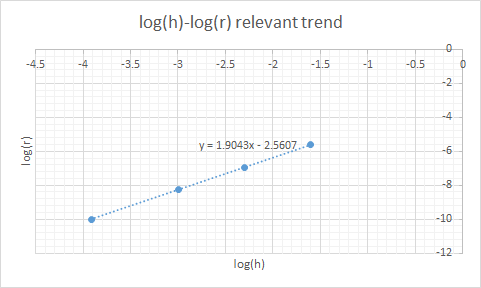
\includegraphics[scale = 0.8]{images/convergence.png}
\caption{The relevance between log(h) and log(r) when $nu=1$.  Mesh
  dimensions are $h=0.2,\ 0.1, \ 0.05, \ 0.02$ and the numerical error
  $r=||u_h-u||_2$. log(h) and log(r) shows linear correlation and the
  slope is 1.9043.}
\label{im::log(h)-res}
\end{figure}

Figure (\ref{im::log(h)-res}) shows the relevance between log(h) and
log(r) when $nu=1$, which the numerical error $r=||u_h-u||_2$. From
the figure the linear correlation of log(h) and log(r) is found and
the slope is 1.9043. That agree with the analytic result of the
convergence order $O(h^2)$.

And for the cavity flow cases, under same boundary value as
(\ref{bd::value1}), we compare the numerical results between
Navier-Stokes fluid and Stokes fluid when
$\nu=1,\ 0.1,\ 0.01,\ h=0.05$ if figure
(\ref{im::Navier-Stoke-solution}).  We can see that the fluids are not
symmetric again. With the viscosity growing, the Moffatt eddies become
more unstable. The bottom right corner eddy catches more energy from
the prime eddy. We continue calculating until the viscosity comes to
0.001. If the viscosity becomes too smaller, the process actully doesn't
converge with the current linear solver. New method is needed.

\begin{figure}[h]
\centering
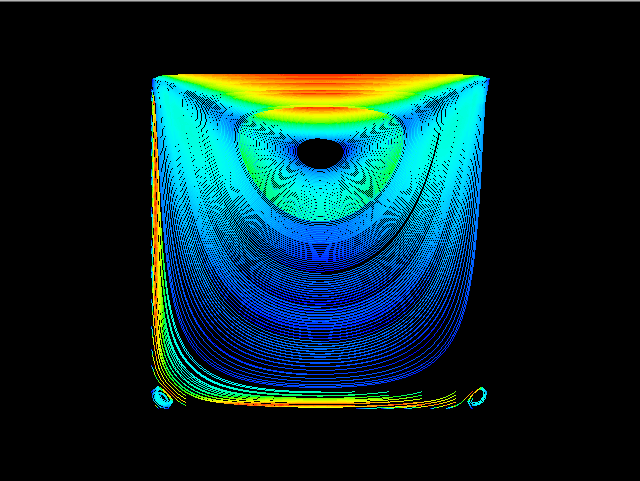
\includegraphics[scale = 0.2]{images/a.png}
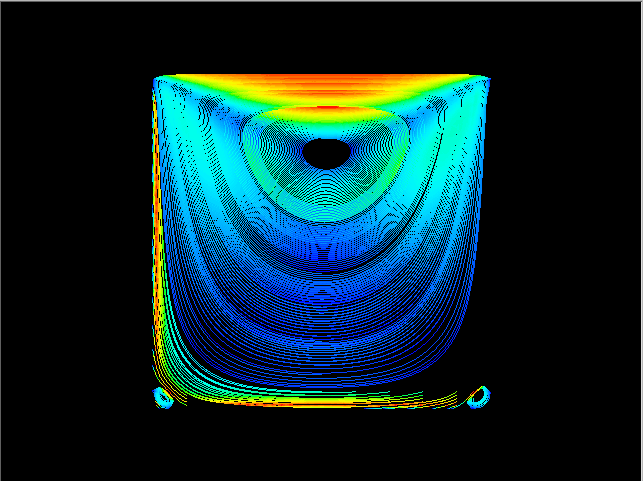
\includegraphics[scale = 0.2]{images/b.png}
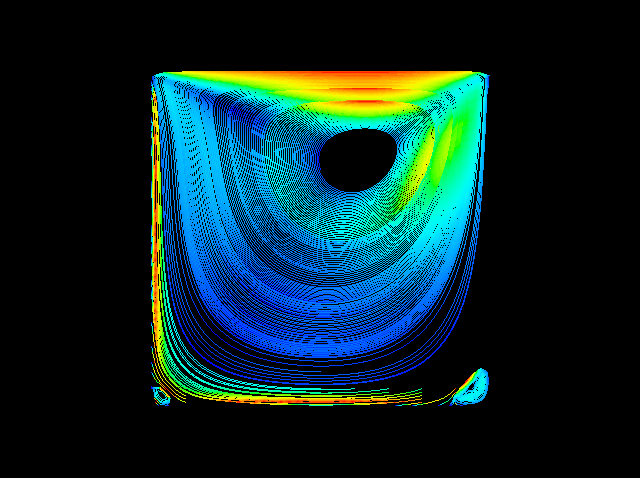
\includegraphics[scale = 0.2]{images/c.png}
\caption{Navier-Stokes Solutions when $\nu$=1, 0.1, 0.01. The fluid becomes more asymmetry and bottom left corner catches more energy.}
\label{im::Navier-Stoke-solution}
\end{figure}

\subsection{Time Depending}
Consider the equations that
\begin{equation}
\begin{array}{rcl}
\frac{\partial\vec{u}}{\partial t}-\nu \nabla^2 \vec{u} + \vec{u}\cdot \nabla \vec{u} + \nabla p &=& \vec{F} \\
\nabla \cdot \vec{u} &=& \vec{0}
\label{eq::Timedepending-problem}
\end{array}
\end{equation}
We add a time-control term to Navier-Stokes equations. If the $\Delta t$ is small enough, the solution will converge to the Navier-Stokes solution under same boundary value.


We use implicit format that $\frac{\partial u}{\partial t} = \frac{u^{n+1}-u^{n}}{\Delta t}$ in $x$ and $y$ directions.
The iteration becomes that
\begin{equation}
\left[ \begin{array}{ccc}
A + N +W_{xx} + T_x & W_{xy} & B_x^T \\
W_{yx} & A +N +W{yy} + T_y& B_y^T \\
B_x & B_y & 0
\end{array}
\right]
\left[\begin{array}{ccc}
\Delta u_x\\
\Delta u_y\\
\Delta p
\end{array}
\right]=
\left[\begin{array}{ccc}
f_x + t_x\\
f_y + t_y\\
g
\end{array}
\right]
\label{Timedepending}
\end{equation}
where $T$ is the $n_u\times n_u$ time mass-matrix.
\begin{equation}
T = [t_{ij}],\quad t_{ij}=\frac{1}{\Delta t}\int_{\Omega}\vec{\phi}_i\cdot\vec{\phi}_j,
\end{equation}
and the vector $t$ is the former velocity value
\begin{equation}
t = [t_{k}],\quad t_{k}=\frac{1}{\Delta t}\int_{\Omega}\vec{u}_h\cdot\vec{\phi}_i.
\end{equation}
\\


This simulation is to solve the Navier-Stokes equations while $\nu=0.00005(Re=2000)$. The solution is that
\begin{figure}[h]
\centering
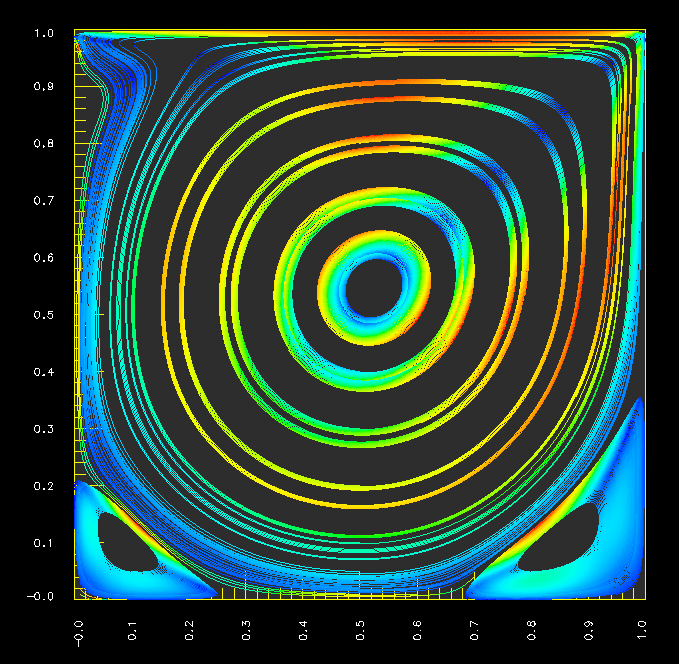
\includegraphics[scale = 0.5]{images/e.png}
\caption{Navier-Stokes solution, the stream lines of the velocity field, the square domain is $[0, 1] \times [0, 1]$ with mesh dimension $h=0.05$ and $\nu=0.00005$. The eddies become larger and new eddy comes to appear.}
\label{im::d}
\end{figure}


In the figure (\ref{im::d}), new eddy comes to appear and the fluid becomes unstable. When the Re($\frac{1}{\nu}$) grows again, the model can't explain the phenomenon any more. It needs to introduce more theories.
\section{Future Work}
\subsection{Three-dimensional calculation}
Actually we just calculate the equations in the plane. For actual calculation, we should extend it to three-dimensional space. The matrix form (\ref{Navier-Stokes}) is rewritten as
\begin{equation}
\left[ \begin{array}{cccc}
A + N +W_{xx} & W_{xy} & W_{xz} & B_x^T \\
W_{yx} & A +N +W{yy}& W_{yz} & B_y^T \\
W_{zx} & W_{zy}  &A + N + W_{zz} & B_z^T \\
B_x & B_y &B_z& 0
\end{array}
\right]
\left[\begin{array}{cccc}
\Delta u_x\\
\Delta u_y\\
\Delta u_z\\
\Delta p
\end{array}
\right]=
\left[\begin{array}{cccc}
f_x\\
f_y\\
f_z\\
g
\end{array}
\right].
\label{3D-Navier-Stokes}
\end{equation}
But new 3D mesh-building tool is required in computer calculating.
\subsection{Precondition}
With the matrix size growing, better precondition is needed. Considering the time-depending Navier-Stokes equations (\ref{eq::Timedepending-problem}), we use semi-implicit scheme that
\begin{equation}
\begin{array}{rcl}
\frac{\vec{u}^{n+1}-\vec{u}^n}{\Delta t} - \nu \nabla^2 \vec{u}^{n+1} + \vec{u}^{n}\cdot \nabla \vec{u}^n + \nabla p^{n+1} &=& \vec{F} \\
\nabla \cdot \vec{u}^{n+1} &=& \vec{0}
\label{eq::implicit and explicit}
\end{array}
\end{equation}
Thus we change the equations to a time-developinig Stokes equations. Now we can use proper precondition like AMG block precondition given before to make the calculating more efficient.

\bibliographystyle{alpha}
\bibliography{sample}

\end{document}
